
\documentclass[a4paper,11pt]{article}%,twocolumn
%% packages

\usepackage{blindtext} % needed for creating dummy text passages
%\usepackage{ngerman} % needed for German default language
\usepackage{amsmath} % needed for command eqref
\usepackage{amssymb} % needed for math fonts
\usepackage[colorlinks=true,breaklinks]{hyperref} % needed for creating hyperlinks in the document, the option colorlinks=true gets rid of the awful boxes, breaklinks breaks lonkg links (list of figures), and ngerman sets everything for german as default hyperlinks language
\usepackage[hyphenbreaks]{breakurl} % ben�tigt f�r das Brechen von URLs in Literaturreferenzen, hyphenbreaks auch bei links, die �ber eine Seite gehen (mit hyphenation).
\usepackage{xcolor}
\definecolor{c1}{rgb}{0,0,1} % blue
\definecolor{c2}{rgb}{0,0.3,0.9} % light blue
\definecolor{c3}{rgb}{0.3,0,0.9} % red blue
\hypersetup{
    linkcolor={c1}, % internal links
    citecolor={c2}, % citations
    urlcolor={c3} % external links/urls
}
%\usepackage{cite} % needed for cite
\usepackage[square,authoryear]{natbib} % needed for cite and abbrvnat bibliography style
\usepackage[nottoc]{tocbibind} % needed for displaying bibliography and other in the table of contents
\usepackage{graphicx} % needed for \includegraphics 
\usepackage{longtable} % needed for long tables over pages
\usepackage{bigstrut} % needed for the command \bigstrut
\usepackage{enumerate} % needed for some options in enumerate
%\usepackage{todonotes} % needed for todos
\usepackage{makeidx} % needed for creating an index
\makeindex
\usepackage{gensymb}
\usepackage{url}
\usepackage{psfrag}
\usepackage{multirow}
\usepackage{subfigure}
%% page settings

\usepackage[top=20mm, bottom=20mm,left=15mm,right=15mm]{geometry} % needed for page border settings
\parindent=0mm % for space of first line of new text block
\sloppy % for writing with hyphenless justification (tries to)
\hyphenation{} % use hyphenation of tolerance parametershttp://www.jr-x.de/publikationen/latex/tipps/zeilenumbruch.html
\hyphenpenalty=10000
\exhyphenpenalty=10000
\usepackage{fancyhdr} % needed for head and foot options
%% my macros

%% Text fomats
\newcommand{\tbi}[1]{\textbf{\textit{#1}}}

%% Math fonts
\newcommand{\bbA}{\mathbb{A}}
\newcommand{\bbB}{\mathbb{B}}
\newcommand{\bbC}{\mathbb{C}}
\newcommand{\bbD}{\mathbb{D}}
\newcommand{\bbE}{\mathbb{E}}
\newcommand{\bbF}{\mathbb{F}}
\newcommand{\bbG}{\mathbb{G}}
\newcommand{\bbH}{\mathbb{H}}
\newcommand{\bbI}{\mathbb{I}}
\newcommand{\bbJ}{\mathbb{J}}
\newcommand{\bbK}{\mathbb{K}}
\newcommand{\bbL}{\mathbb{L}}
\newcommand{\bbM}{\mathbb{M}}
\newcommand{\bbN}{\mathbb{N}}
\newcommand{\bbO}{\mathbb{O}}
\newcommand{\bbP}{\mathbb{P}}
\newcommand{\bbQ}{\mathbb{Q}}
\newcommand{\bbR}{\mathbb{R}}
\newcommand{\bbS}{\mathbb{S}}
\newcommand{\bbT}{\mathbb{T}}
\newcommand{\bbU}{\mathbb{U}}
\newcommand{\bbV}{\mathbb{V}}
\newcommand{\bbW}{\mathbb{W}}
\newcommand{\bbX}{\mathbb{X}}
\newcommand{\bbY}{\mathbb{Y}}
\newcommand{\bbZ}{\mathbb{Z}}


% Define colors
\definecolor{codegreen}{rgb}{0,0.6,0}
\definecolor{codegray}{rgb}{0.5,0.5,0.5}
\definecolor{codepurple}{rgb}{0.58,0,0.82}
\definecolor{backcolour}{rgb}{0.95,0.95,0.92}
% Setup the listings package
\lstset{
    backgroundcolor=\color{backcolour},   
    commentstyle=\color{codegreen},
    keywordstyle=\color{magenta},
    numberstyle=\tiny\color{codegray},
    stringstyle=\color{codepurple},
    basicstyle=\footnotesize,
    breakatwhitespace=false,         
    breaklines=true,                 
    captionpos=b,                    
    keepspaces=true,                 
    numbers=left,                    
    numbersep=5pt,                  
    showspaces=false,                
    showstringspaces=false,
    showtabs=false,                  
    tabsize=2
}



\begin{document}
\begin{titlepage}
\center % Center everything on the page

%-------------------------------------------------------------------------------------
%	HEADING SECTIONS
%------------------------------------------------------------------------------------
\textbf{\large Department of Electrical and Computer Engineering}\\[0.5cm]
\textbf{\Large University of Colorado at Boulder}\\[1cm]
\textbf{\large ECEN5730 - Practical PCB design}\\[2cm]

\includegraphics[width=0.3\textwidth]{figures/cu}\\[2cm] 

	
%-------------------------------------------------------------------------------------
%	TITLE SECTION
%------------------------------------------------------------------------------------

\textbf{\Huge Board Good Layout/Bad Layout }\\[0.2cm]

\textbf{\Large Report}\\[2cm]
\vspace{1.5cm}
\begin{figure}[H]
	\centering
	
\includegraphics[scale=0.2]{figures/qr_download.png}
	\label{555_schematic}
\end{figure}\vspace{1.5cm}


%----------------------------------------------------------------------------------------
%	MEMBERS SECTION
%----------------------------------------------------------------------------------------


\vfill

\textbf{\large Submitted by}

{\large Parth Thakkar}\\[0.5cm]




%----------------------------------------------------------------------------------------
%	DATE SECTION
%----------------------------------------------------------------------------------------

\textbf{\large Submitted on}\\
\textbf{\Large \today} % Date, change the \today to a set date if you want to be precise

%----------------------------------------------------------------------------------------

\vfill % Fill the rest of the page with whitespace

\end{titlepage}

\pagebreak

\tableofcontents
\listoffigures
\listoftables
\vfill
\begin{center}
	\textbf{\textit{*PDF is clickable}}
\end{center}

\pagebreak

\section{Objective / Purpose of Lab}
\begin{enumerate}
	\item One of the key parameters used to characterize VRMs is the Thevenin equivalent circuit model. The Thevenin model represents a voltage source as a combination of an ideal voltage source (Thevenin voltage, VTH) and a series resistance (Thevenin resistance, RTH). This model is particularly useful for analyzing the behavior of VRMs under varying load conditions, as the output voltage and current will depend on the values of VTH and RTH, as well as the load resistance.
	\item 
	\item The objective of this lab is to design, build, and test a custom instrument, the "Instrument Droid," capable of measuring the Thevenin parameters (VTH and RTH) of various voltage sources and regulators as a function of the output current load. By sweeping the load current and measuring the corresponding output voltages, the Instrument Droid can determine the Thevenin voltage (the open-circuit voltage) and the Thevenin resistance (the slope of the voltage-current curve).

	\item To precisely control the voltage across the sense resistor, and consequently the current through the MOSFET, an external digital-to-analog converter (DAC) is utilized. The DAC, in this case, the MCP4725, receives digital inputs from an Arduino microcontroller and generates an analog voltage output proportional to the desired current level.

	\item the Instrument Droid incorporates a high-resolution analog-to-digital converter (ADC), specifically the ADS1115, to measure the voltage across the sense resistor and the loaded output voltage of the VRM. By employing differential voltage measurement techniques, the ADC can accurately capture the voltage drops across the sense resistor and the VRM, even in the presence of noise or ground offsets.

	\item To account for potential power dissipation issues, especially when characterizing high-current VRMs, the Instrument Droid implements a pulsed current measurement approach. By applying short current pulses with low duty cycles, the average power dissipation in the circuit components can be maintained within safe operating limits, preventing overheating and potential damage.
\end{enumerate}



% \begin{figure}[H]
% 	\centering
% 	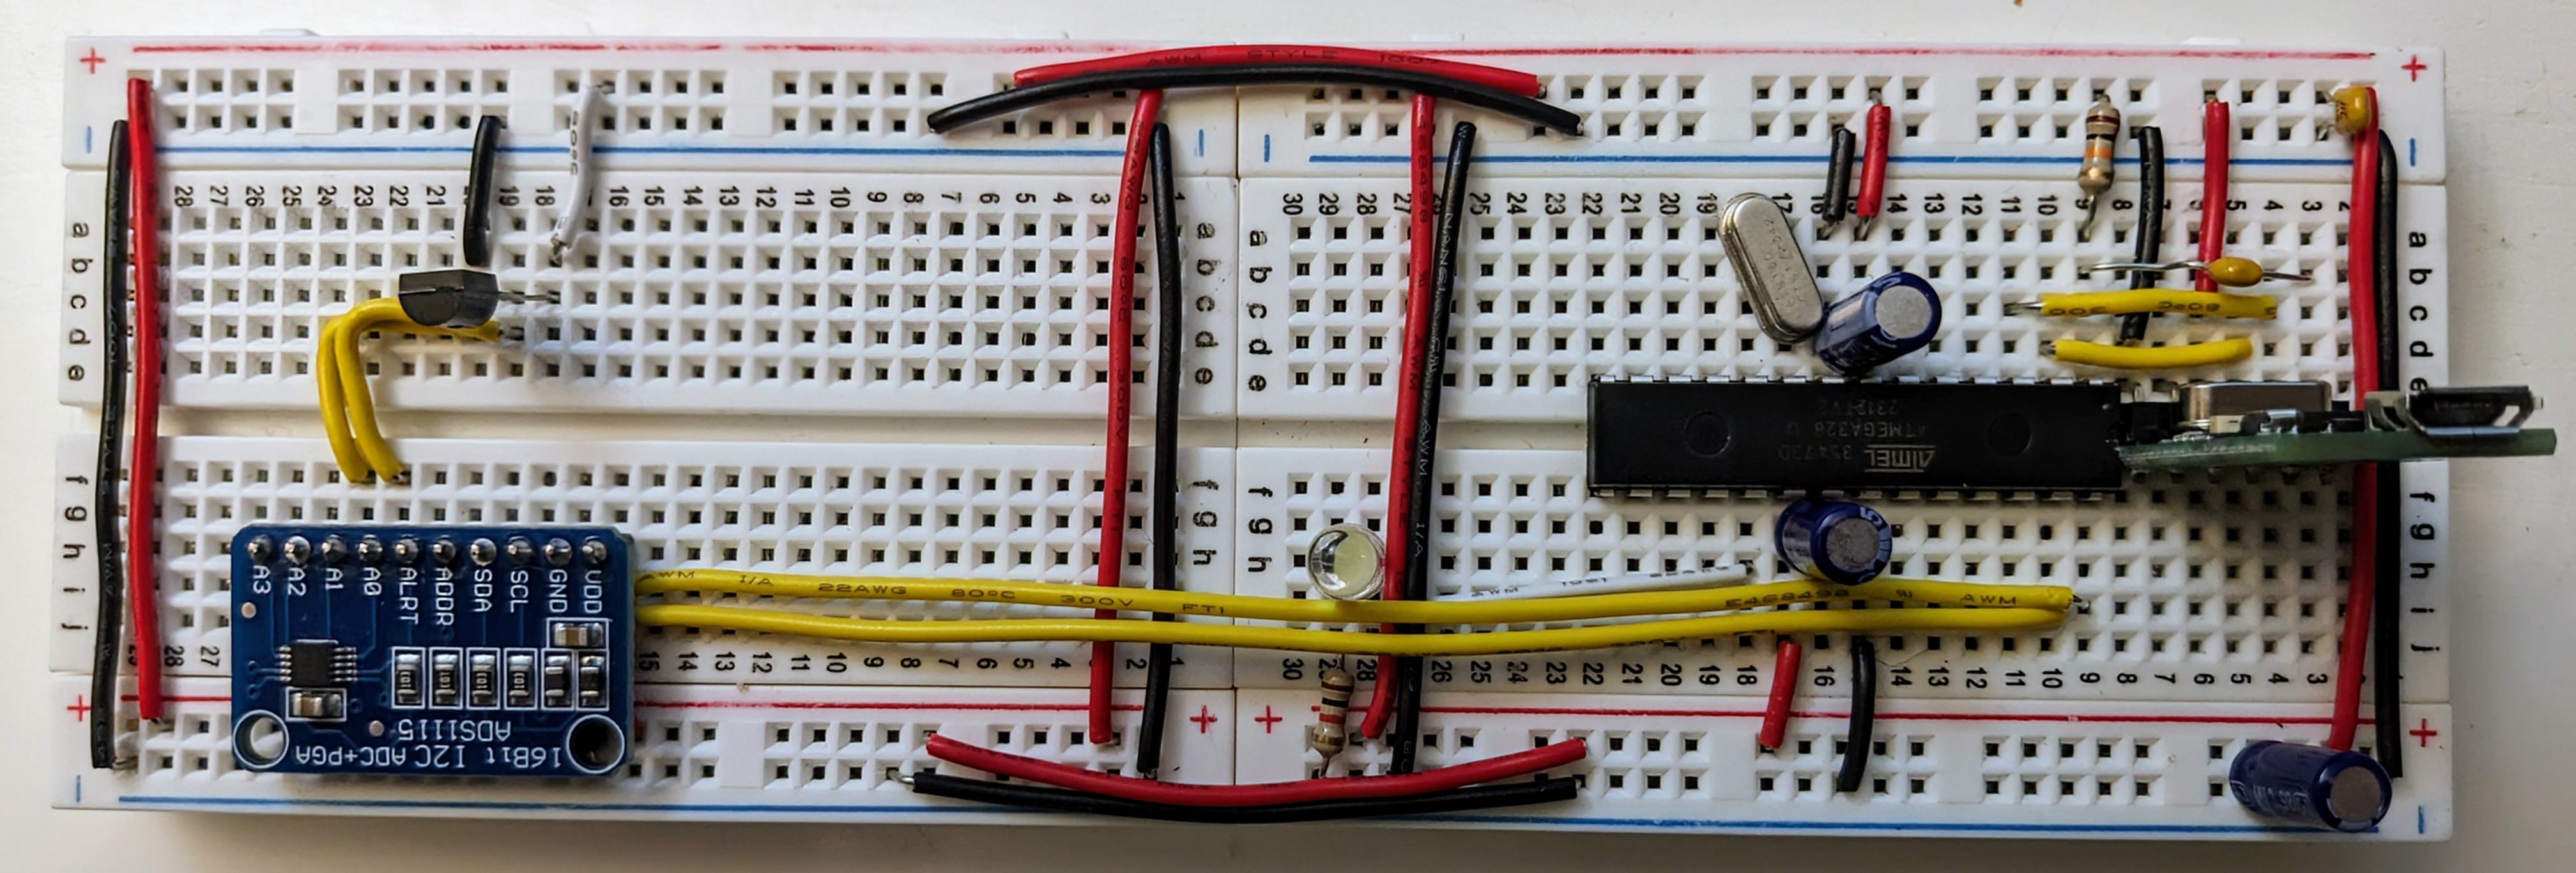
\includegraphics[scale=0.10]{figures/breadboard.jpg}
% 	\caption{Breadboard implementation}
% \end{figure}

% \begin{figure}[H]
% 	\centering
% 	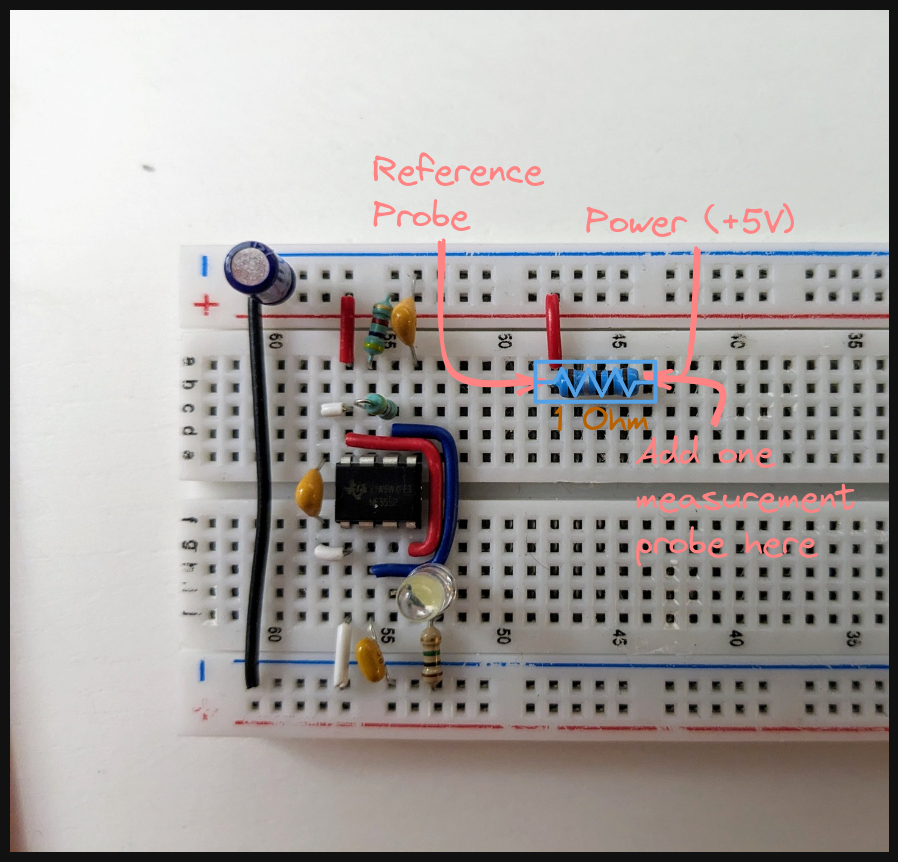
\includegraphics[scale=0.40]{figures/setup.png}
% 	\caption{Setup}
% \end{figure}

% \begin{figure}[H]
% 	\centering
% 	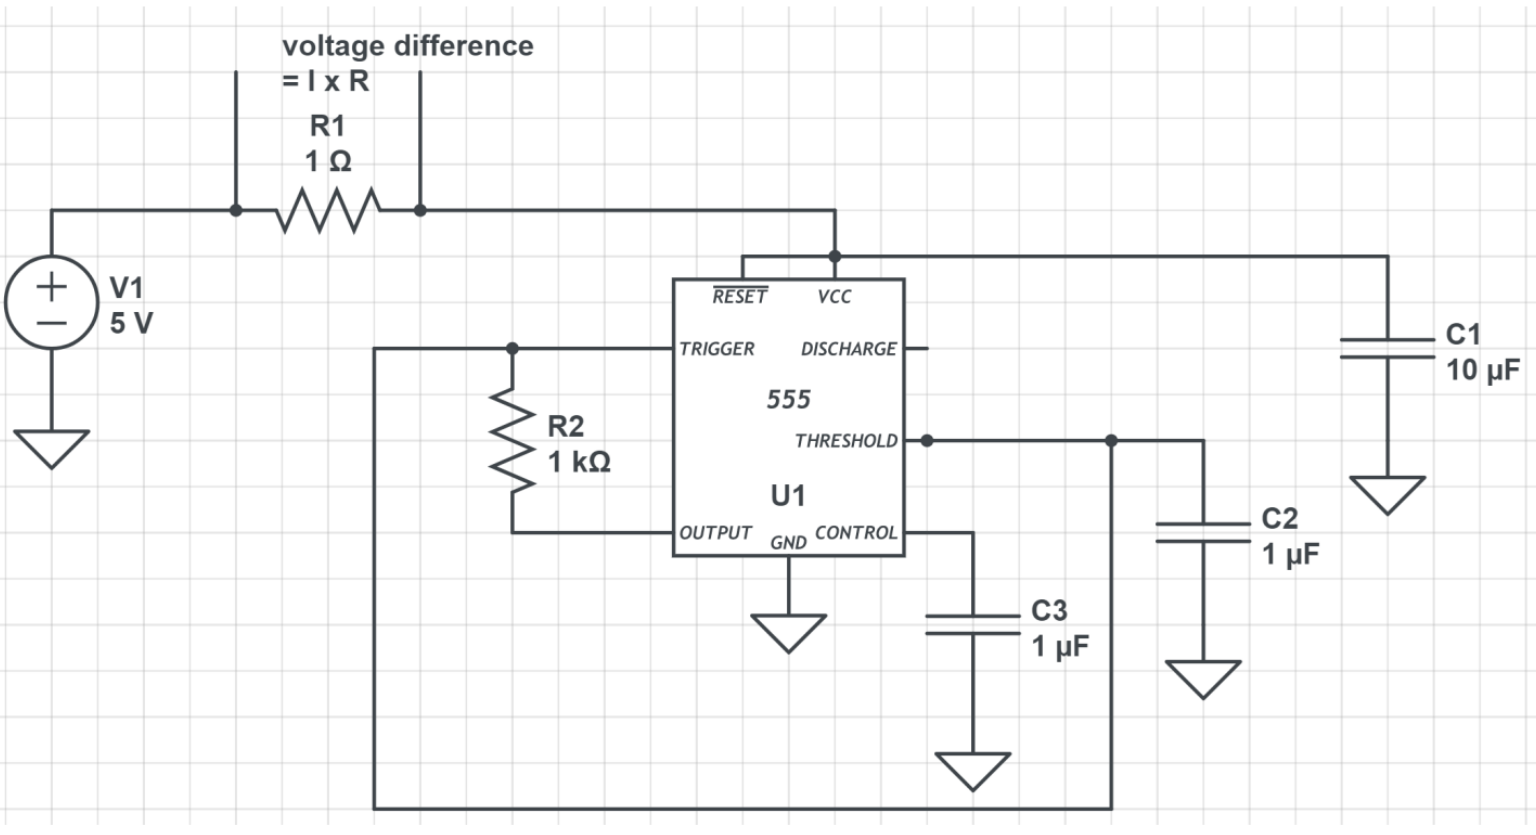
\includegraphics[scale=0.30]{figures/block_diagram.png}
% 	\caption{Block Diagram}
% \end{figure}


\section{Component listing}



\begin{table}[H]
\centering
\caption{Component Listing}
\begin{tabular}{|l|l|l|}
\hline
\textbf{Component} & \textbf{Description} & \textbf{Quantity} \\ \hline
Arduino Uno & Microcontroller board & 1 \\ \hline
MCP4725 & 12-bit DAC & 1 \\ \hline
ADS1115 & 16-bit ADC & 1 \\ \hline
MOSFET (IRL520) & Electronic load & 1 \\ \hline
Op-amp (MCP601) & Operational amplifier & 1 \\ \hline
Sense resistor & Current sense resistor (10 $\ohm$) & 1 \\ \hline
Resistors & Voltage divider resistors & 2 \\ \hline
Breadboard & Solderless breadboard & 1 \\ \hline
Jumper wires & Connection wires & As needed \\ \hline
\end{tabular}
\end{table}



\section{Explanation}

\begin{figure}[H]
	\centering
	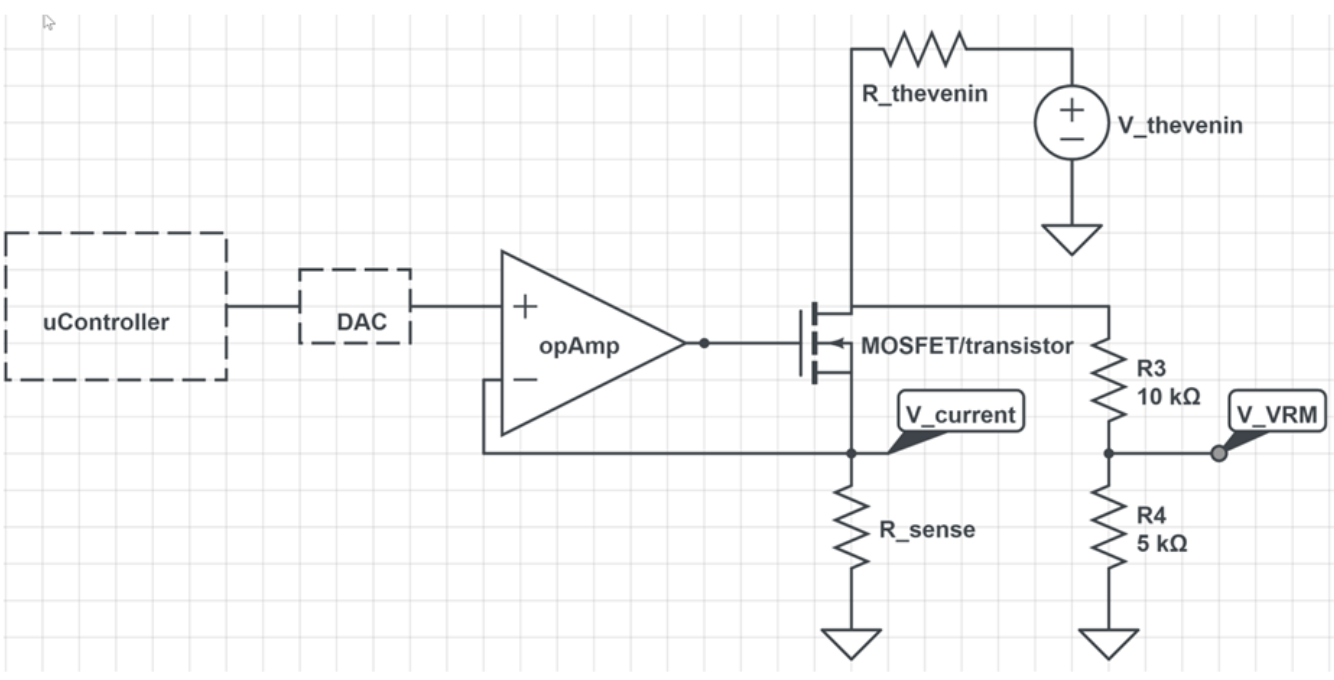
\includegraphics[scale=0.38]{figures/vrm_block_diagram.png}
  \caption{Block diagram}
\end{figure}
\begin{itemize}

  \item In this circuit configuration, the operational amplifier (op-amp) is crucial for its role in controlling the MOSFET as a voltage-controlled current source. The op-amp is set up in a non-inverting configuration, where its output is fed back to its inverting input through a voltage divider formed by R3 and R4. This feedback loop allows the op-amp to adjust its output voltage to match the input voltage, effectively functioning as a voltage follower.
  \item The DAC, controlled by a microcontroller, generates an analog voltage proportional to the desired current level. This voltage signal is applied to the non-inverting input of the op-amp, serving as the reference voltage for the op-amp's negative feedback loop. That is why we are giving it stable output thorough DAC IC
  \item we are using voltage divider for measuring VRM voltage as ADS1115 is only capable of measuring 5 V , voltage sources higher than 5 v will burn the ADS11115 that is why we are using voltage divider
  \item In this circuit, V\_current and V\_VRM are used to measure the current through the VRM and the VRM's output voltage, respectively. These measurements are essential for determining the Thevenin equivalent of the VRM.
  \item Measuring V\_current (Voltage across R\_sense):\\
  The voltage across the sense resistor (R\_sense) is directly proportional to the current flowing through it, according to Ohm's law: V = I x R. By measuring the voltage across R\_sense using the microcontroller's ADC and knowing the value of R\_sense, we can calculate the current through the VRM:
  \begin{itemize}
    \item I\_VRM = V\_current / R\_sense
    \item This current measurement allows us to characterize the VRM's behavior under different load conditions.
  \end{itemize}
  \item Measuring V\_VRM:\\
  V\_VRM represents the output voltage of the VRM. However, the VRM's output voltage may be too high for the microcontroller's ADC to measure directly. To overcome this, a voltage divider consisting of resistors R3 and R4 is used to scale down the VRM voltage to a level suitable for the ADC.
  The scaled VRM voltage (V\_VRM\_scaled) is given by:
  \begin{itemize}
    \item V\_VRM\_scaled = V\_VRM $\cdot$ $\frac{R4}{(R3 + R4)}$
    \item By measuring V\_VRM\_scaled using the ADC and knowing the values of R3 and R4, we can calculate the actual VRM output voltage:
    \item V\_VRM = V\_VRM\_scaled $\cdot$ $\frac{(R3 + R4)}{R4}$
  \end{itemize}
  \item Op-amp usage:\\
  \begin{itemize}
    \item The op-amp in this circuit is configured as a non-inverting amplifier, which serves as a voltage-controlled current source (VCCS) for the MOSFET. The DAC output voltage is applied to the non-inverting input of the op-amp, and the inverting input is connected to the sense resistor (R\_sense).
  
    \item The op-amp tries to maintain the same voltage at both its inputs by adjusting its output voltage. This forces the voltage across R\_sense to be equal to the DAC output voltage. As a result, the current through R\_sense, and consequently the current through the MOSFET and VRM, is controlled by the DAC output voltage.
    
    \item The op-amp also provides a high input impedance, ensuring that it doesn't load the DAC output, and a low output impedance, enabling it to drive the MOSFET gate effectively.
  \end{itemize}
  \item MOSFET usage:\\
  \begin{itemize}
    \item The MOSFET acts as a voltage-controlled current source in this circuit. The op-amp output voltage, which is controlled by the DAC, is applied to the MOSFET's gate. The MOSFET's drain current (I\_D) is proportional to the gate-source voltage (V\_GS) when operating in the saturation region.
  
    \item By varying the DAC output voltage, the op-amp adjusts the MOSFET's gate voltage, thus controlling the current through the MOSFET and, consequently, the current through the VRM. This allows the microcontroller to set different load currents and measure the VRM's response.
    
    \item The MOSFET is chosen for its high input impedance, which minimizes loading on the op-amp output, and its ability to handle large currents required for characterizing the VRM.
  \end{itemize}
\end{itemize}


In summary, the op-amp and MOSFET work together as a voltage-controlled current source to regulate the current through the VRM, while V\_current and V\_VRM measurements provide the necessary data for determining the VRM's Thevenin equivalent.

\begin{lstlisting}
	// vrm characterizer board
#include <Wire.h>
#include <Adafruit_MCP4725.h>
Adafruit_MCP4725 dac;
float DAC_ADU_per_v = 4095.0 / 5.0;  //conversion from volts to ADU
int V_DAC_ADU;                       // the value in ADU to output on the DAC

void setup() {
  Serial.begin(115200);
  dac.begin(0x60);           // address is either 0x60, 0x61, 0x62,0x63, 0x64 or 0x65
  dac.setVoltage(0, false);  //sets the output current to 0 initially
}




void loop() {
  // put your main code here, to run repeatedly:
  V_DAC_ADU = 0 * DAC_ADU_per_v;
  dac.setVoltage(V_DAC_ADU, false);  //sets the output current to 0 initially
  V_DAC_ADU = 3.0 * DAC_ADU_per_v;
  dac.setVoltage(V_DAC_ADU, false);  //sets the output current to 0 initially
}
\end{lstlisting}

\begin{lstlisting}
	// vrm characterizer board
#include <Wire.h>
#include <Adafruit_MCP4725.h>
#include <Adafruit_ADS1X15.h>

Adafruit_ADS1115 ads;
Adafruit_MCP4725 dac;
float R_sense = 10.0;                      //current sensor
long itime_on_msec = 100;                  //on time for taking measurements
long itime_off_msec = itime_on_msec * 10;  // time to cool off
int iCounter_off = 0;                      // counter for number of samples off
int iCounter_on = 0;                       // counter for number of samples on
float v_divider = 5000.0 / 15000.0;        // voltage divider on the VRM
float DAC_ADU_per_v = 4095.0 / 5.0;        //conversion from volts to ADU
int V_DAC_ADU;                             // the value in ADU to output on the DAC
int I_DAC_ADU;                             // the current we want to output
float I_A = 0.0;                           // the current we want to output, in amps
long itime_stop_usec;                      // this is the stop time for each loop
float ADC_V_per_ADU = 0.125 * 1e-3;        // the voltage of one bit on the gain of 1 scale
float V_VRM_on_v;                          // the value of the VRM voltage
float V_VRM_off_v;                         // the value of the VRM voltage
float I_sense_on_A;                        // the current through the sense resistor
float I_sense_off_A;                       // the current through the sense resistor
float I_max_A = 0.25;                      // max current to set for
int npts = 20;                             //number of points to measure
float I_step_A = I_max_A / npts;           //step current change


float I_load_A;  // the measured current load
float V_VRM_thevenin_v;
float V_VRM_loaded_v;
float R_thevenin;
int i;


void setup() {
  Serial.begin(115200);
  dac.begin(0x60);           // address is either 0x60, 0x61, 0x62,0x63, 0x64 or 0x65
  dac.setVoltage(0, false);  //sets the output current to 0 initially


  // ads.setGain(GAIN_TWOTHIRDS); // 2/3x gain +/- 6.144V 1 bit = 3mV     0.1875mV (default)
  ads.setGain(GAIN_ONE);  // 1x gain   +/- 4.096V 1 bit = 2mV     0.125mV
  // ads.setGain(GAIN_TWO);       // 2x gain   +/- 2.048V 1 bit = 1mV     0.0625mV
  // ads.setGain(GAIN_FOUR);      // 4x gain   +/- 1.024V 1 bit = 0.5mV   0.03125mV
  // ads.setGain(GAIN_EIGHT);     // 8x gain   +/- 0.512V 1 bit = 0.25mV  0.015625mV
  // ads.setGain(GAIN_SIXTEEN);   // 16x gain  +/- 0.256V 1 bit = 0.125mV 0.0078125mV
  ads.begin();                           // note- you can put the address of the ADS111 here if needed
  ads.setDataRate(RATE_ADS1115_860SPS);  // sets the ADS1115 for higher speed
}


void loop() {
  for (i = 1; i <= npts; i++) {
    I_A = i * I_step_A;
    dac.setVoltage(0, false);  //sets the output current
    func_meas_off();
    func_meas_on();
    dac.setVoltage(0, false);  //sets the output current


    I_load_A = I_sense_on_A - I_sense_off_A;  //load current
    V_VRM_thevenin_v = V_VRM_off_v;
    V_VRM_loaded_v = V_VRM_on_v;
    R_thevenin = (V_VRM_thevenin_v - V_VRM_loaded_v) / I_load_A;
    // if (V_VRM_loaded_v < 0.75 * V_VRM_thevenin_v) i = npts;  //stops the ramping


    Serial.print(i);
    Serial.print(", ");
    Serial.print(I_load_A * 1e3, 3);
    Serial.print(", ");
    Serial.print(V_VRM_thevenin_v, 4);
    Serial.print(", ");
    Serial.print(V_VRM_loaded_v, 4);
    Serial.print(", ");
    Serial.println(R_thevenin, 4);
  }
  Serial.println("done");
  delay(30000);
}



void func_meas_off() {
  dac.setVoltage(0, false);  //sets the output current
  iCounter_off = 0;          //starting the current counter

  V_VRM_off_v = 0.0;  //initialize the VRM voltage averager

  I_sense_off_A = 0.0;  // initialize the current averager

  itime_stop_usec = micros() + itime_off_msec * 1000;  // stop time
  while (micros() <= itime_stop_usec) {
    V_VRM_off_v = ads.readADC_Differential_0_1() * ADC_V_per_ADU / v_divider + V_VRM_off_v;
    I_sense_off_A = ads.readADC_Differential_2_3() * ADC_V_per_ADU / R_sense + I_sense_off_A;
    iCounter_off++;
  }
  V_VRM_off_v = V_VRM_off_v / iCounter_off;
  I_sense_off_A = I_sense_off_A / iCounter_off;
  // Serial.print(iCounter_off);Serial.print(", ");
  // Serial.print(I_sense_off_A * 1e3, 4); Serial.print(", ");
  // Serial.println(V_VRM_off_v, 4);
}


void func_meas_on() {
  //now turn on the current
  I_DAC_ADU = I_A * R_sense * DAC_ADU_per_v;
  dac.setVoltage(I_DAC_ADU, false);  //sets the output current
  iCounter_on = 0;
  V_VRM_on_v = 0.0;                                   //initialize the VRM voltage averager
  I_sense_on_A = 0.00;                                // initialize the current averager
  itime_stop_usec = micros() + itime_on_msec * 1000;  // stop time

  while (micros() <= itime_stop_usec) {
    V_VRM_on_v = ads.readADC_Differential_0_1() * ADC_V_per_ADU / v_divider + V_VRM_on_v;
    I_sense_on_A = ads.readADC_Differential_2_3() * ADC_V_per_ADU / R_sense + I_sense_on_A;
    iCounter_on++;
  }
  dac.setVoltage(0, false);
  //sets the output current to zero
  V_VRM_on_v = V_VRM_on_v / iCounter_on;
  I_sense_on_A = I_sense_on_A / iCounter_on;
  // Serial.print(iCounter_on);Serial.print(", ");
  // Serial.print(I_sense_on_A * 1e3, 4);Serial.print(", ");
  // Serial.println(V_VRM_on_v, 4);
}
\end{lstlisting}


Here's a breakdown of the code:
\begin{itemize}
  \item It iterates over a specified number of points (npts) with increasing load currents (I\_A).
  For each iteration: a. It calls func\_meas\_off() to measure the VRM voltage (V\_VRM\_off\_v) and current (I\_sense\_off\_A) when no load is applied. b. It calls func\_meas\_on() to apply the desired load current (I\_A) and measure the corresponding VRM voltage (V\_VRM\_on\_v) and current (I\_sense\_on\_A). c. It calculates the load current (I\_load\_A), Thevenin equivalent voltage (V\_VRM\_thevenin\_v), loaded VRM voltage (V\_VRM\_loaded\_v), and Thevenin resistance (R\_thevenin). d. It prints the measurement results (iteration, load current, Thevenin voltage, loaded voltage, Thevenin resistance). e. It checks if the loaded VRM voltage drops below 75\% of the Thevenin voltage. If so, it stops the ramping process (i = npts) because the VRM is unable to supply more current without significant voltage drop.
  \item The func\_meas\_off() and func\_meas\_on() functions handle the actual measurement process:
  \begin{itemize}
    \item func\_meas\_off() sets the DAC output to 0 (no load), then takes multiple samples of the VRM voltage and current over a specified time period (itime\_off\_msec). It averages the samples to obtain V\_VRM\_off\_v and I\_sense\_off\_A.
    \item func\_meas\_on() sets the DAC output to apply the desired load current (I\_DAC\_ADU), then takes multiple samples of the VRM voltage and current over a specified time period (itime\_on\_msec). It averages the samples to obtain V\_VRM\_on\_v and I\_sense\_on\_A.
    \item The reason for stopping the ramping process when the loaded VRM voltage drops below 75\% of the Thevenin voltage is to prevent excessive loading of the VRM, which could potentially damage it or cause unreliable measurements. This threshold is a safety measure to ensure that the VRM is not pushed beyond its capable current delivery range.
  \end{itemize}
  
  \item By measuring the Thevenin voltage and resistance at different load currents, this code can characterize the behavior of the VRM, including its output impedance, current-handling capability, and any non-linear effects that may occur at higher currents.
\end{itemize}



\section{Measurement}

The Instrument Droid was used to characterize various voltage sources and regulators, including known sources for verification purposes and unknown sources to demonstrate the instrument's capabilities. This section presents the measurement results and analyses for each source.

\subsection{Function Generator as a Known Source} 

To verify the proper operation of the Instrument Droid, a function generator was initially used as a known voltage source. The function generator was set to provide a constant DC voltage output, and its Thevenin parameters were calculated based on the manufacturer's specifications \& previous labs.\\

Expected Thevenin Resistance (RTH): 50$\ohm$\\

The Instrument Droid was then used to measure the function generator's output voltage and current at various load conditions. The measured data was processed to determine the Thevenin parameters, and the results were compared to the expected values.\\

Measured Value\\
\boxed{Thevenin Resistance (RTH)	: 49.82$\ohm$}\\
The measured Thevenin voltage and resistance closely matched the expected values, confirming the accurate operation of the Instrument Droid.\\

\ref{fig:vrm_block_diagram} shows the plot of the measured Thevenin resistance versus the output current for the function generator.\\

\begin{figure}[H]
	\centering
	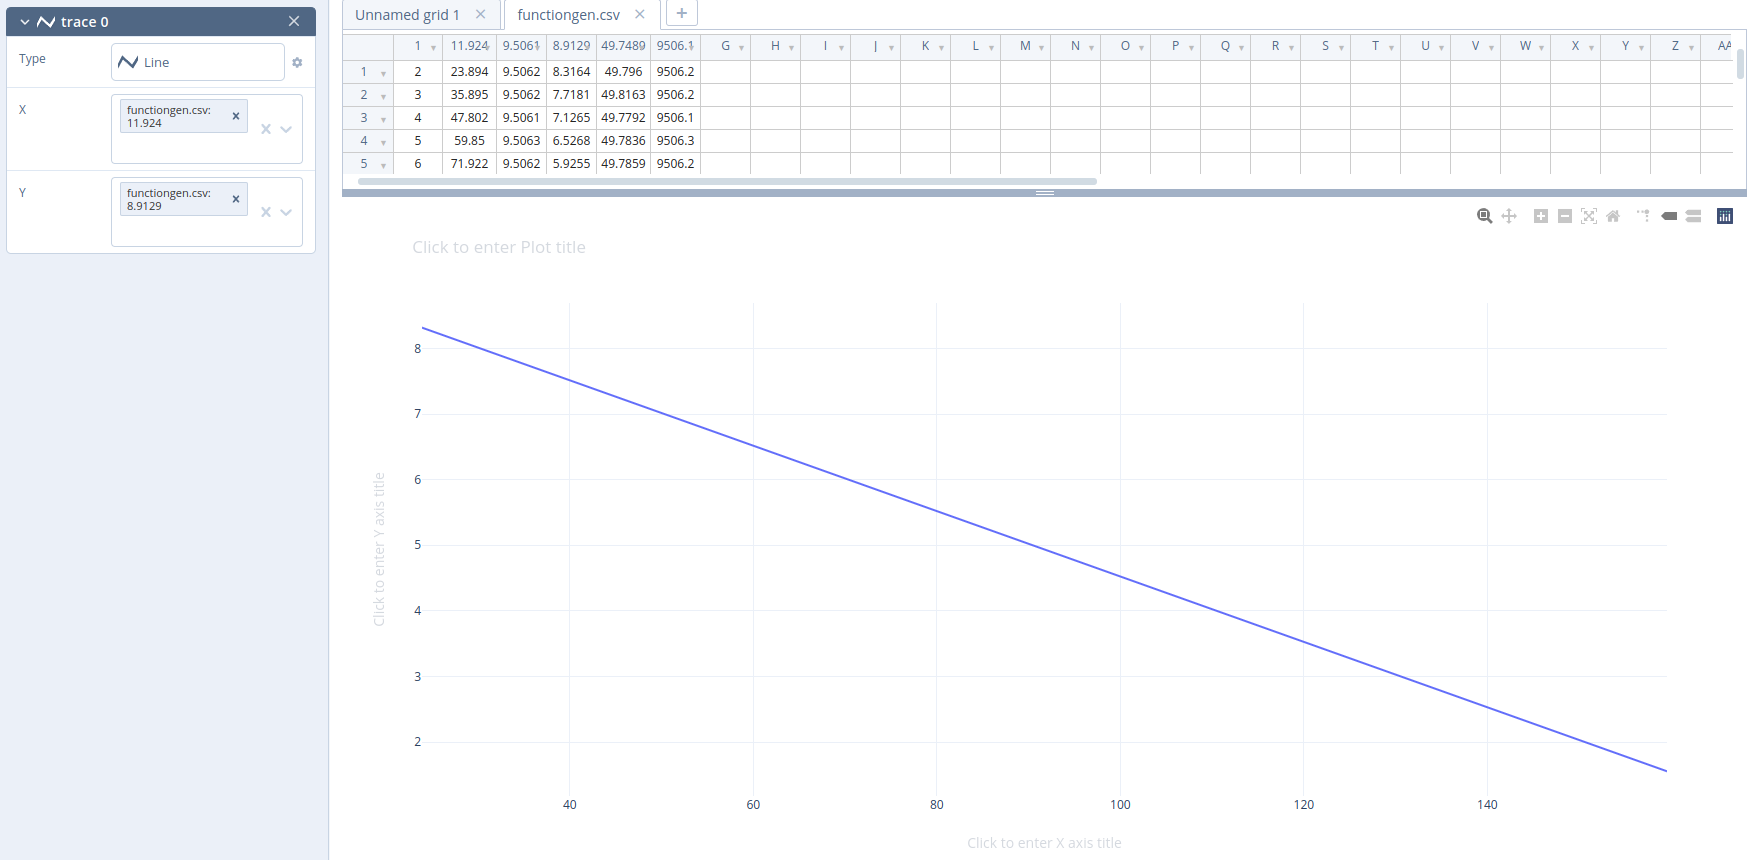
\includegraphics[scale=0.30]{figures/function_generator.png}
  \caption{Current vs Voltage for function generator}
  \label{fig:function_generator}
\end{figure}

As expected, the Thevenin resistance remained relatively constant across the measured current range, consist  ent with the low output impedance of the function generator, slope of this graph gives us R\_th which is 50ohm in our case

\begin{lstlisting}
function generator output:
1, 11.924, 9.5061, 8.9129, 49.7489 
2, 23.894, 9.5062, 8.3164, 49.7960 
3, 35.895, 9.5062, 7.7181, 49.8163 
4, 47.802, 9.5061, 7.1265, 49.7792 
5, 59.850, 9.5063, 6.5268, 49.7836 
6, 71.922, 9.5062, 5.9255, 49.7859 
7, 83.958, 9.5060, 5.3261, 49.7859 
8, 96.045, 9.5060, 4.7236, 49.7944 
9, 107.803, 9.5060, 4.1337, 49.8350 
10, 119.821, 9.5059, 3.5365, 49.8195 
11, 131.941, 9.5061, 2.9306, 49.8362 
12, 143.925, 9.5061, 2.3353, 49.8233 
13, 155.883, 9.5060, 1.7387, 49.8279 
14, 159.550, 9.5062, 1.5550, 49.8350 
15, 159.550, 9.5062, 1.5548, 49.8361 
16, 159.560, 9.5060, 1.5548, 49.8322 
17, 159.565, 9.5060, 1.5546, 49.8319 
18, 159.568, 9.5062, 1.5551, 49.8290 
19, 159.568, 9.5061, 1.5551, 49.8286 
20, 159.570, 9.5060, 1.5554, 49.8254 
done
\end{lstlisting}





\subsection{Bench Power Supply} 

Expected Value	of RTH \\
Thevenin Resistance (RTH)		1$\ohm$ to 5$\ohm$ \\

The Instrument Droid was then used to measure the Voltage Supply set at 5V  voltage and current at various load conditions. The measured data was processed to determine the Thevenin parameters, and the results were compared to the expected values.\\


Measured Value\\
\boxed{Thevenin Resistance (RTH)	: 0.95$\ohm$}\\
The measured Thevenin voltage and resistance closely matched the expected values, confirming the accurate operation of the Instrument Droid.\\


Figure 2 shows the plot of the measured Thevenin resistance versus the output current for the modified bench power supply.\\


\begin{figure}[H]
	\centering
	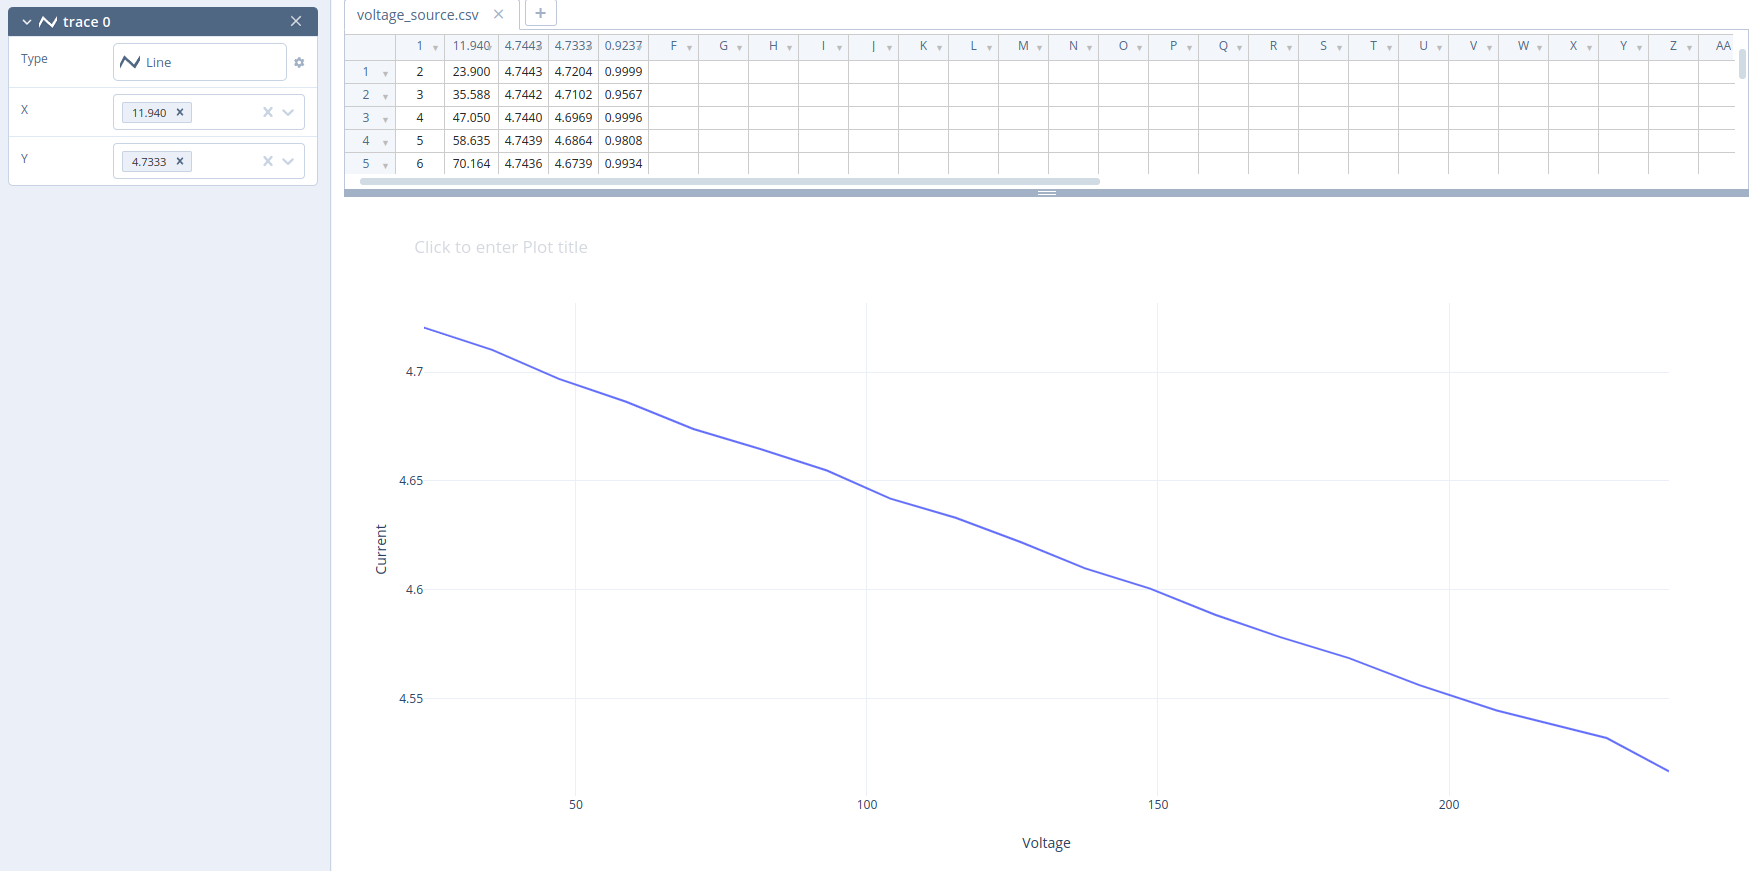
\includegraphics[scale=0.30]{figures/vs.png}
  \caption{Current vs Voltage Source Graph for Function generator}
  \label{fig:vs}
\end{figure}

As anticipated, the Thevenin resistance remained relatively constant across the measured current range, reflecting the combined resistance of the power supply's output impedance and the added series resistor.

\begin{lstlisting}
Voltage source
1, 11.940, 4.7443, 4.7333, 0.9237
2, 23.900, 4.7443, 4.7204, 0.9999 
3, 35.588, 4.7442, 4.7102, 0.9567
4, 47.050, 4.7440, 4.6969, 0.9996
5, 58.635, 4.7439, 4.6864, 0.9808
6, 70.164, 4.7436, 4.6739, 0.9934
7, 81.665, 4.7434, 4.6647, 0.9644
8, 93.135, 4.7434, 4.6548, 0.9515
9, 104.004, 4.7434, 4.6419, 0.9763
10, 115.224, 4.7435, 4.6331, 0.9585
11, 126.478, 4.7435, 4.6219, 0.9615
12, 137.464, 4.7436, 4.6099, 0.9731
13, 148.660, 4.7436, 4.6006, 0.9624
14, 159.808, 4.7435, 4.5886, 0.9689
15, 171.008, 4.7437, 4.5783, 0.9670
16, 182.815, 4.7437, 4.5687, 0.9571
17, 194.903, 4.7438, 4.5563, 0.9618
18, 208.189, 4.7437, 4.5446, 0.9560
19, 227.082, 4.7439, 4.5320, 0.9333
20, 237.792, 4.7439, 4.5167, 0.9553
done
\end{lstlisting}

\subsection{Bench Power Supply with Known Resistance} 

To further validate the Instrument Droid's measurements, a bench power supply was used with a known series resistor added. This configuration allowed for a predictable Thevenin resistance to be measured.\\

Added Series Resistor: 10$\ohm$ \\
Expected Thevenin Resistance (RTH): 1$\ohm$ +10$\ohm$  = 11$\ohm$ \\

Measured Value	\\
\boxed{Thevenin Resistance 11$\ohm$} \\
The measured Thevenin voltage and resistance closely matched the expected values, further confirming the accuracy of the Instrument Droid's measurements.\\

Figure \ref{vs10} shows the plot of the measured Thevenin resistance versus the output current for the modified bench power supply.\\


\begin{figure}[H]
	\centering
	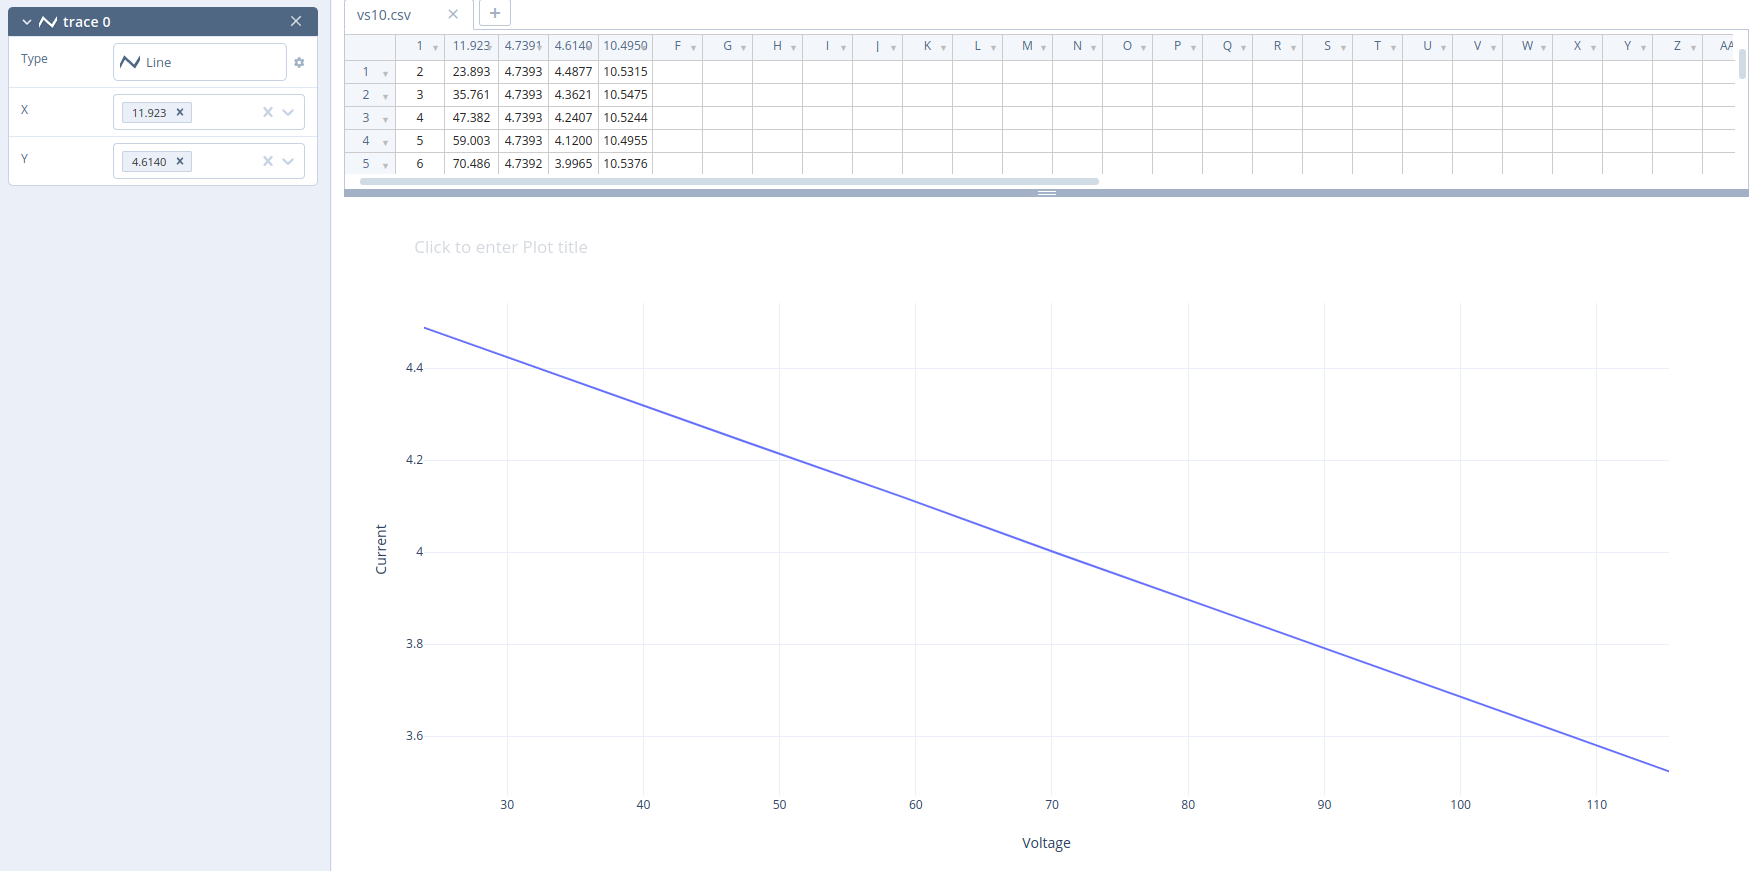
\includegraphics[scale=0.30]{figures/vs10.png}
  \caption{current vs Voltage for Voltage Source with 10$\ohm$ added}
  \label{fig:vs10}
\end{figure}

As anticipated, the Thevenin resistance remained relatively constant across the measured current range, reflecting the combined resistance of the power supply's output impedance and the added series resistor.

\begin{lstlisting}
1, 11.923, 4.7391, 4.6140, 10.4950
2, 23.893, 4.7393, 4.4877, 10.5315
3, 35.761, 4.7393, 4.3621, 10.5475
4, 47.382, 4.7393, 4.2407, 10.5244
5, 59.003, 4.7393, 4.1200, 10.4955
6, 70.486, 4.7392, 3.9965, 10.5376
7, 81.636, 4.7393, 3.8793, 10.5348
8, 92.688, 4.7395, 3.7631, 10.5339
9, 103.668, 4.7393, 3.6467, 10.5395
20, 115.301, 4.7393, 3.5235, 10.5442
done
\end{lstlisting}

\subsection{Unknown Voltage Sources} 

After verifying the Instrument Droid's operation with known sources, various unknown voltage sources and regulators were characterized. These sources included wall warts, batteries, Arduino outputs, op-amp outputs, and other voltage sources commonly found in electronics laboratories.\\

For each unknown source, the Instrument Droid measured the output voltage and current at various load conditions. The measured data was processed to determine the Thevenin parameters, and the results were analyzed to gain insights into the source's behavior.\\

\subsubsection{5V Wall Wart} 


The first unknown source measured was a 5V wall wart power adapter. The Instrument Droid was used to sweep the load current and measure the corresponding output voltages.\\\\

Parameter	Measured Value\\
Thevenin Voltage (VTH)	4.5V\\
\boxed{Thevenin Resistance (RTH)	0.9553$\ohm$ }\\
Figure \ref{5vsupply} shows the plot of the measured Thevenin resistance versus the output current for the 5V wall wart.\\


\begin{figure}[H]
	\centering
	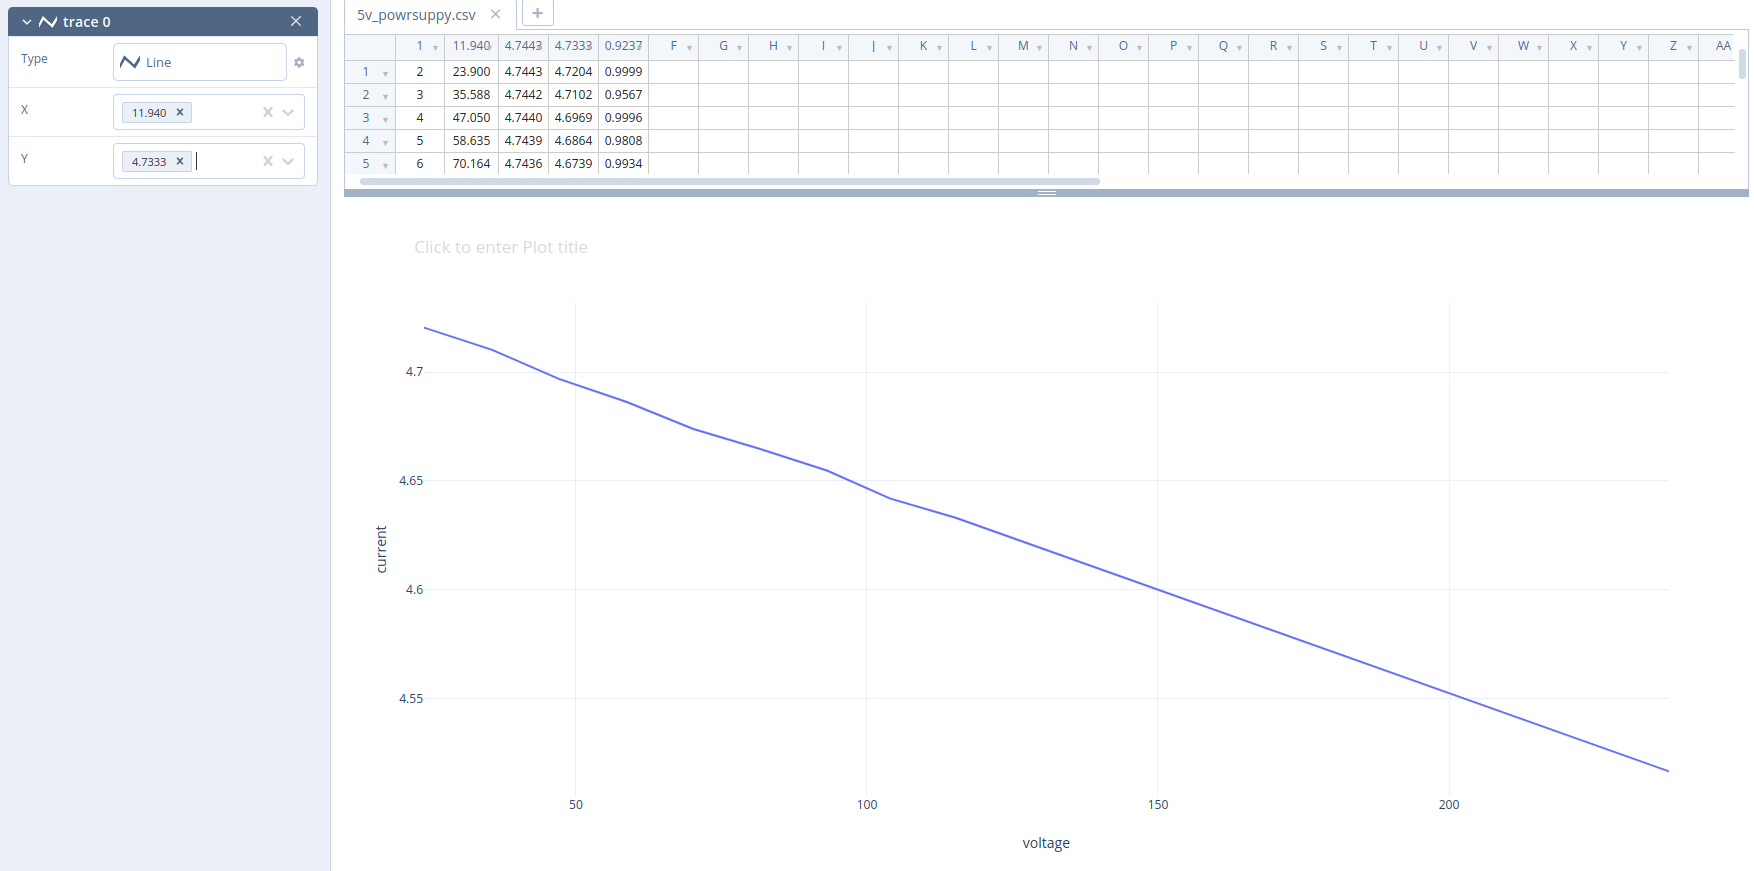
\includegraphics[scale=0.30]{figures/5v.png}
  \caption{Voltage vs Current analysis 5V supply}
  \label{fig:5vsupply}
\end{figure}

Analysis and observations:\\
Slope of the graph gives us R\_th for the 5v wall power supply, from the graph we can see that the R\_th is around 1$\ohm$ which matches the output of instrument droid


\begin{lstlisting}
1, 11.940, 4.7443, 4.7333, 0.9237
2, 23.900, 4.7443, 4.7204, 0.9999 
3, 35.588, 4.7442, 4.7102, 0.9567
4, 47.050, 4.7440, 4.6969, 0.9996
5, 58.635, 4.7439, 4.6864, 0.9808
6, 70.164, 4.7436, 4.6739, 0.9934
7, 81.665, 4.7434, 4.6647, 0.9644
8, 93.135, 4.7434, 4.6548, 0.9515
9, 104.004, 4.7434, 4.6419, 0.9763
10, 115.224, 4.7435, 4.6331, 0.9585
20, 237.792, 4.7439, 4.5167, 0.9553
\end{lstlisting}

\subsubsection{9V battery} 


The second unknown source measured was a 9V wall Battery. The Instrument Droid was used to sweep the load current and measure the corresponding output voltages.\\

Measured Value\\
\boxed{Thevenin Resistance (RTH)	17$\ohm$} \\
Figure \ref{9vsuppy} shows the plot of the measured Thevenin resistance versus the output current for the 5V wall wart.\\


\begin{figure}[H]
	\centering
	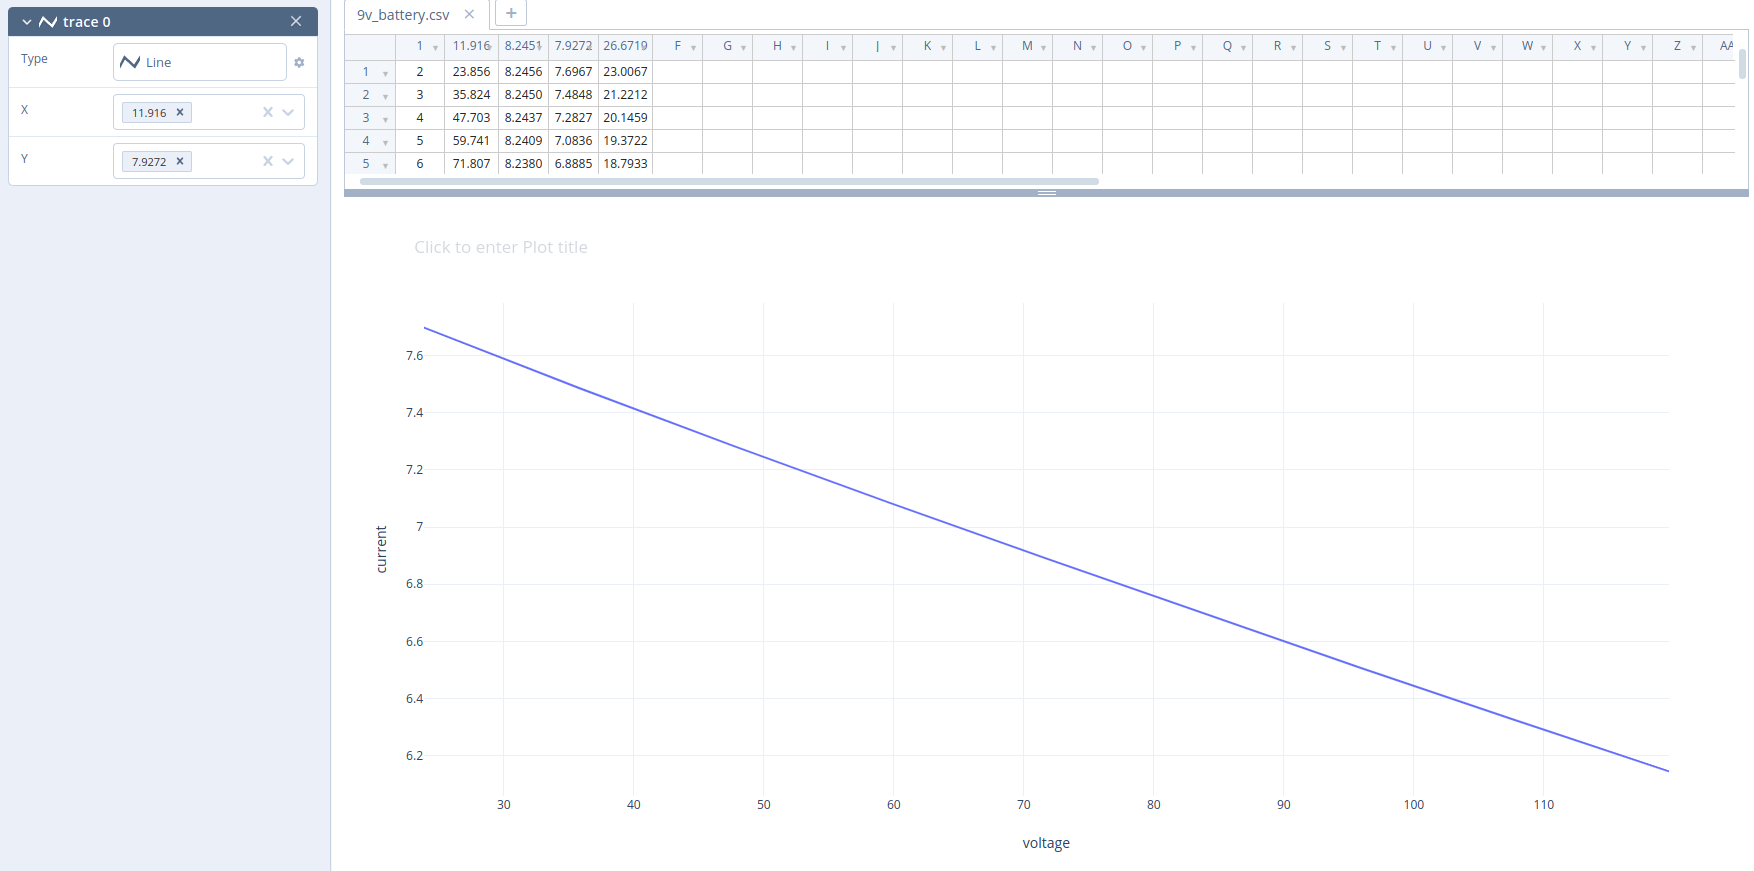
\includegraphics[scale=0.30]{figures/9v.png}
  \caption{Current vs Voltage for 9V supply}
  \label{fig:9vsuppy}
\end{figure}

Analysis and observations:\\
Slope of the graphs gives us 17$\ohm$  which matches our R\_th output of the instrument droid


\begin{lstlisting}
1, 11.916, 8.2451, 7.9272, 26.6719 
2, 23.856, 8.2456, 7.6967, 23.0067 
3, 35.824, 8.2450, 7.4848, 21.2212 
4, 47.703, 8.2437, 7.2827, 20.1459 
5, 59.741, 8.2409, 7.0836, 19.3722 
6, 71.807, 8.2380, 6.8885, 18.7933 
7, 83.825, 8.2347, 6.6979, 18.3336 
8, 95.877, 8.2314, 6.5083, 17.9723 
9, 107.644, 8.2274, 6.3271, 17.6537 
20, 119.629, 8.2231, 6.1461, 17.3624 
done
\end{lstlisting}


\begin{figure}[H]
	\centering
	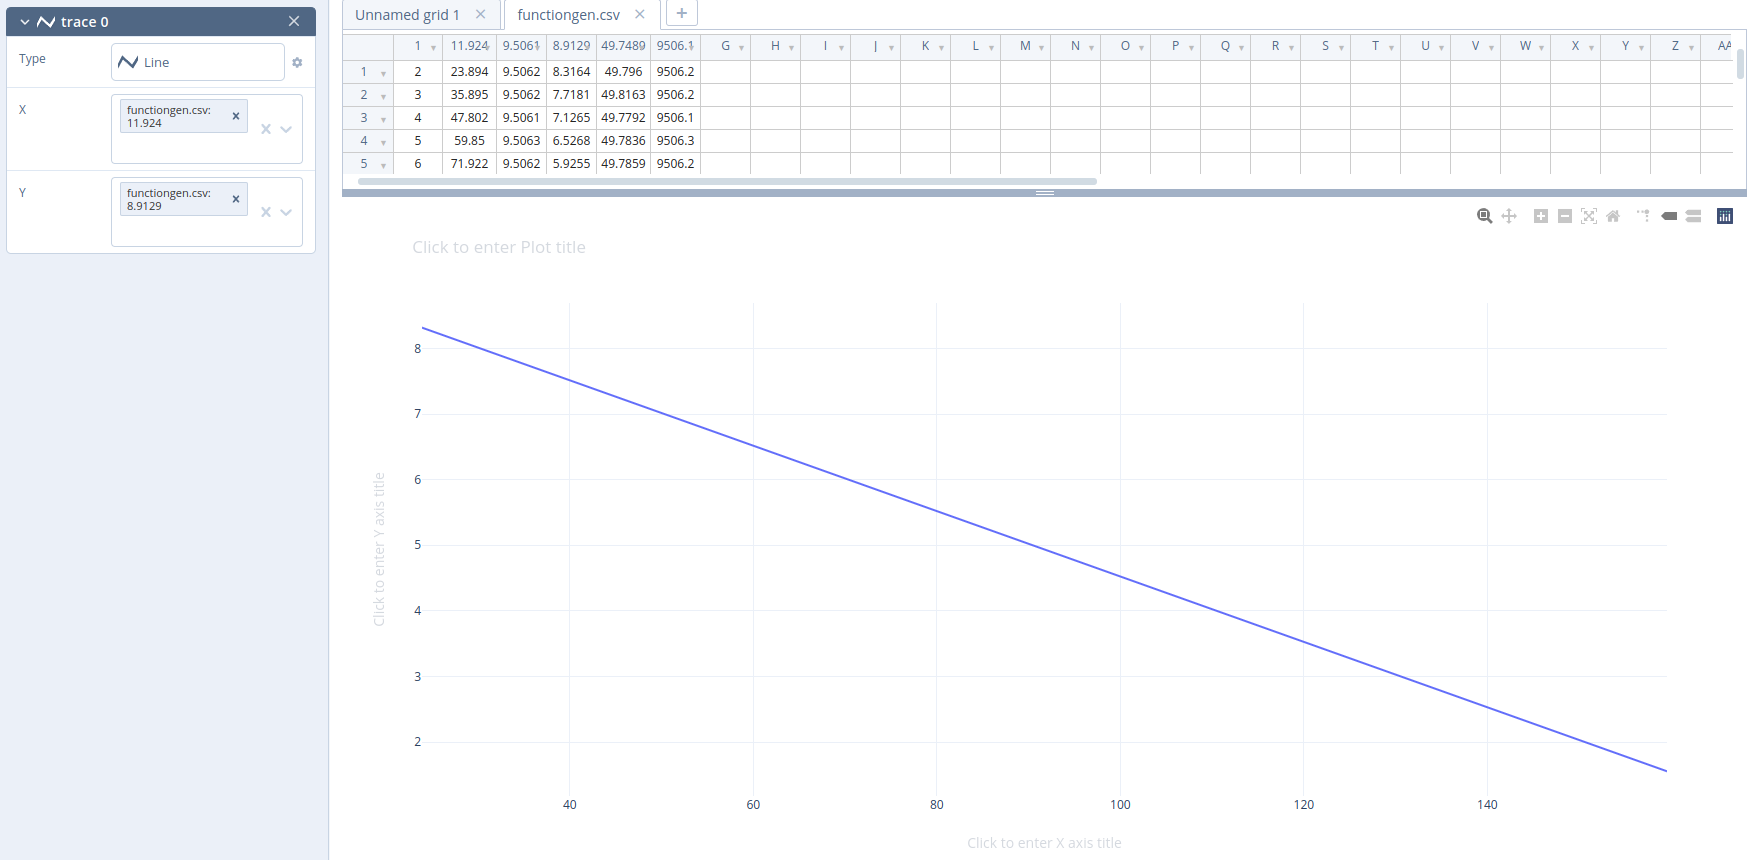
\includegraphics[scale=0.30]{figures/function_generator.png}
  \caption{Block diagram}
  \label{fig:vrm_block_diagram}
\end{figure}


\section{Learnings and Observation}
\begin{enumerate}
  \item Practical circuit design and implementation: The lab provided hands-on experience in designing and constructing a custom instrument (Instrument Droid) for characterizing voltage sources and regulators. This involved selecting appropriate components, considering power dissipation, and implementing measurement techniques, reinforcing the importance of careful design and analysis.
  \item Integration of multiple subsystems: The Instrument Droid involved the integration of various subsystems, including a microcontroller, DAC, ADC, op-amp, and MOSFET. Coordinating the operations of these subsystems and ensuring proper interfacing and communication was a valuable learning experience in system integration and design.
  \item Noise management and signal conditioning: The lab highlighted the impact of noise and signal integrity on measurements. Techniques such as differential voltage measurement and proper grounding practices were essential for obtaining accurate and reliable results, reinforcing the importance of noise management and signal conditioning in electronic circuit design.
  \item Data analysis and visualization: The lab involved collecting and processing measurement data, calculating parameters, and plotting the results. This reinforced the importance of data analysis, visualization, and interpretation in characterizing and understanding the behavior of electronic systems.
\end{enumerate}





\section{Conclusion}

\begin{enumerate}
  \item The Instrument Droid proved to be an effective tool for characterizing voltage sources and regulators by measuring their Thevenin parameters. By sweeping the load current and measuring the corresponding output voltages, the Instrument Droid could accurately determine the Thevenin voltage and Thevenin resistance.
  \item Verification with known sources, such as a function generator and a bench power supply with a known series resistor, confirmed the accurate operation of the Instrument Droid. This approach allowed for the identification and resolution of any potential issues before proceeding to characterize unknown sources.
  \item The Instrument Droid successfully characterized various unknown voltage sources, including wall warts, batteries, Arduino outputs, op-amp outputs, and other voltage sources commonly found in electronics laboratories. The measured Thevenin parameters and resistance curves provided valuable insights into the behavior and characteristics of these sources under varying load conditions.
  \item Comparing the measured Thevenin parameters and resistance curves with theoretical expectations or manufacturer specifications for well-understood voltage sources, such as batteries and regulated power supplies, allowed for further investigation and discussion, deepening the understanding of the underlying principles and potential sources of error.
  \item The pulsed current measurement approach implemented in the Instrument Droid effectively managed power dissipation, preventing overheating and potential damage to circuit components, especially when characterizing high-current voltage sources.
  \item The lab experience reinforced the importance of a systematic approach, attention to detail, and the ability to analyze and interpret data in the context of theoretical principles and practical considerations when designing and testing electronic circuits and instrumentation systems.
\end{enumerate}







\vspace{50px}
\hrule
\hrule

\pagebreak





%---------------------------------------------------------------------------
\end{document}

